\chapter[Singular values: Expansion amplitudes]{Singular values:\\ Expansion amplitudes}

\section{Introduction}
We have answered the most basic questions about the \svdp \ by showing two different ways to decompose a target matrix. With this requirement satisfied, we will move to more abstract issues. The next several chapters will focus on interpretation of the decomposition components. The goal is to foster an intuition for the domain matrices and the singular values. In particular the singular values are a minor hurdle. Of course the singular values are the square root of the eigenvalues of the product matrices. Yet there is much more that story.

While most of the elaboration will take place part \eqref{pictures} ``The SVD in pictures,'' there is an important analytic piece to resolve first. We will look at the generalized Fourier expansion and compare that to the SVD. We will see that the singular values play the role of the expansion amplitudes which regulate the summation of rank one matrices.

This will open the door to two concepts:
\begin{enumerate}
\item low-rank approximations of matrices, and
\item distance to higher-rank matrices.
\end{enumerate}

%%
\section{Matrix representations}
The are many different expansions we could use to represent a matrix. For example, we could extend the concept of unit vectors to matrices. Consider the arbitrary matrix
\begin{equation}
  \A{} = 
  \mat{cc}{a & b \\c & d} = 
  a \mat{cc}{1 & 0 \\ 0 & 0} +
  b \mat{cc}{0 & 1 \\ 0 & 0} +
  c \mat{cc}{0 & 0 \\ 1 & 0} +
  d \mat{cc}{0 & 0 \\ 0 & 1}.
\end{equation}
While correct, this resolution is not very fulfilling as it does little to shed light on anything more than the most basic structure. For example, we would recognize
\begin{equation}
  a \mat{cc}{1 & 0 \\ 0 & 0} +
  d \mat{cc}{0 & 0 \\ 0 & 1}
\end{equation}
as a diagonal matrix,
\begin{equation}
    \mat{cc}{1 & 0 \\ 0 & 0} +
  b \mat{cc}{0 & 1 \\ 0 & 0} +
    \mat{cc}{0 & 0 \\ 0 & 1}
\end{equation}
as an upper-triangular matrix, etc.

%%%%
\section{Rank one expansion}
We can glean a great deal of information about a matrix by simply looking at the decomposition in terms of column vectors for the domain and codomain matrices. Consider a matrix $\Amnr$ with the standard decomposition products. Let $y_{k}$ be the $k$th column of the codomain matrix $\Y{}$ and $x_{k}$ be the $k$th column of the domain matrix $\X{}$. The target matrix can be written in terms of a sum of outer products created by the column vectors of the domain matrices. Consider the domain matrix to be an orthogonal collection of $n-$vectors and the codomain matrix to be a orthogonal collection of $m-$vectors:
\begin{equation}
  \X{} = \mat{c|c|c}{x_{1} & \dots & x_{n}}, \quad \Y{} = \mat{c|c|c}{y_{1} & \dots & y_{m}}.
\end{equation}
The thin SVD can be cast in terms of these vectors:
\begin{equation}
  \begin{split}
    \svda{*} \\
    &= \mat{c|c|c}{y_{1} & \dots & y_{\rho}} \mat{c}{\sigma_{1} x_{1}^{\TT} \\\hline \vdots \\\hline \sigma_{\rho} x_{\rho}^{\TT}} \\
    &= \sigma_{1} y_{1} x_{1}^{\TT} + \sigma_{2} y_{2} x_{2}^{\TT} + \dots + \sigma_{\rho} y_{\rho} x_{\rho}^{\TT}
  \end{split}
\end{equation}
which we can write more compactly as this
\begin{equation}
  \A{} = \sum_{k=1}^{\rho}{ \sigma_{k} y_{k} x_{k}^{\TT} }.
  \label{eq:45:resolve}
\end{equation}
Some may prefer an explicit, yet equivalent, representation for the outer product:
\begin{equation}
  \A{} = \sum_{k=1}^{\rho}{ \sigma_{k} y_{k} \otimes x_{k} }
\end{equation}
In this relation, the singular values acts like amplitudes regulating a combination of $\rho$ rank one matrices.

Please make sure that the summation formula is crystalline clear before going forward. Some much of what follows build upon crisp understanding of the vector operations in matrix analysis. To gain traction, it may be helpful to work out an example for $\Arrr{2}{2}{2}$. (exercise **).
\cite[p. **]{Laub}


%%%
\section{Fourier expansion}
Let's study the Fourier expansion in $\realm$.\cite[p. 299]{Meyer} Assume that we have a complete set of orthonormal vectors $u$ for the space. We can describe an arbitrary $m-$vector $x$ in terms of these vectors as this:
\begin{equation}
  x = \xi_{1} u_{1} + \xi_{2} u_{2} + \dots + \xi_{m} u_{m}
  \label{eq:45:Fourier}
\end{equation}
where the amplitudes $\xi_{k}$, $k=1,2,\dots m$ are scalars.

In fact these amplitudes are the projection of the vector $x$ onto the space spanned by $u_{k}$:
\begin{equation}
  \xi_{k} = \inner{x,u_{k}} = x\cdot u_{k} = x^{\TT}u, \quad k=1,2,\dots m.
\end{equation}

\begin{figure}[htbp] %  figure placement: here, top, bottom, or page
   \centering
   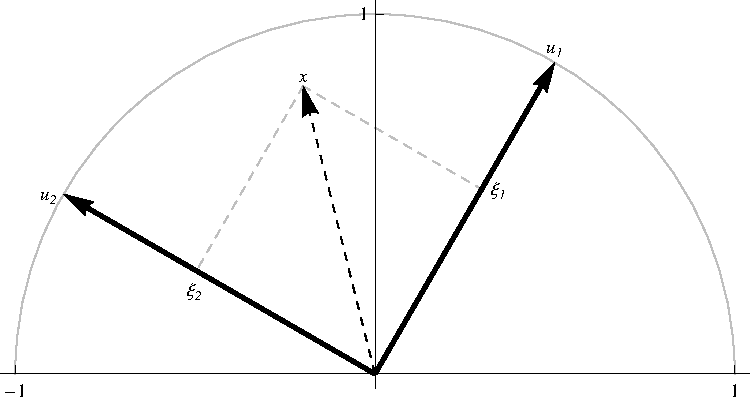
\includegraphics[ ]{pdf/"ch 05"/projections} 
   \caption[A sample projection in $\real{2}$]{A sample projection in $\real{2}$. We see the projections $\xi_{1}$ and $\xi_{2}$ of $x$ onto the orthogonal unit vectors $u_{1}$ and $u_{2}$.}
   \label{fig:45:projections}
\end{figure}

In this case we are projecting vectors onto vectors. Let's extend the concept in equation \eqref{eq:45:Fourier} to project matrices onto matrices. 

In the Fourier expansion, we start with \emph{one} orthonormal set of basis vectors $\lst{u}$, take a \emph{vector} $x$ and compute the amplitudes in a \emph{vector} $\lst{\xi}$.

Now, we will start with \emph{two} orthonormal sets of basis matrices, $\lst{x}$ and $\lst{y}$, take a \emph{matrix} $\A{}$ and compute the amplitudes in a \emph{matrix} $\sig{}$.
\begin{equation}
  \Y{*} \A{} \X{} = \Y{*} \paren{ \svd{*} } \X{} = \sig{}
\end{equation}
So if we have the domain matrices, we do not need to solve an eigenvalue problem to find the singular values. We can use this generalized projection method. This was in essence the method of chapter 1: construct domain matrices and solve for singular values.

Of course, a very good question becomes where do we get the domain matrices from? We usually need to find the \svdl \ in order to find them.

The next step is to apply the projection to the rank one decomposition in equation \eqref{eq:45:resolve}
\begin{equation}
  \begin{split}
     \Y{*}\,\A{}\,\X{} &= \sum_{k=1}^{\rho}{ \sigma_{k} \paren{\Y{*} y_{k} x_{k}^{\TT}\,\X{}}} \\
     &= \sigma_{1} \mat{cccc|c}{ 1 & 0 & \dots & 0 \\ 0 & 0 & \dots & 0 \\ \vdots && \ddots & \\ 0 &&& 0 \\\hline &&&&\zero} \\
     &+  \sigma_{2} \mat{cccc|c}{ 0 & 0 & \dots & 0 \\ 0 & 1 & \dots & 0 \\ \vdots && \ddots & \\ 0 &&& 0 \\\hline &&&&\zero} \\
     &+ \dots \\
     &+ \sigma_{\rho} \mat{cccc|c}{ 0 & 0 & \dots & 0 \\ 0 & 0 & \dots & 0 \\ \vdots && \ddots & \\ 0 &&& 1 \\\hline &&&&\zero}  \\
     &= \sig{}
  \end{split}
\end{equation}
Think of the process as sliding unit entries along the first $\rho$ elements of the sabot matrix.

We have returned to the unit norm matrices in the first section. Except this time we have a rank condition that tells us how much each unit matrix contributes.

Formally, these unit norm matrices are specified using
\begin{equation}
  \B{} = \paren{\Y{*} y_{k} x_{k}^{\TT} \X{}}.
\end{equation}
The entry for row $r$ and column $c$ is given by this
\begin{equation}
  b_{rc} = 
  \begin{cases}
  1 & r=c=k\\
  0 & \text{otherwise}
  \end{cases}.
\end{equation}
We see that $\B{}$ has the same dimension as the target matrix $\A{}$, that is, $\B{}\in\realmn$. With this notation, we can write the following:
\begin{equation}
  \sig{} = \sigma_{1} \B{}_{1} + \sigma_{2} \B{}_{2} + \dots + \sigma_{\rho} \B{}_{\rho} = \sum^{\rho}_{k=1}\sigma_{k} \B{}_{k}.
\end{equation}

To complete the analysis
\begin{equation}
  \begin{split}
    \svda{*} \\
      &= \Y{} \paren{  \sigma_{1} \B{}_{1} + \sigma_{2} \B{}_{2} + \dots + \sigma_{\rho} \B{}_{\rho} } \X{*} \\
      &= \sigma_{1}\, \Y{}\,\B{}_{1}\,\X{*} + \sigma_{2}\, \Y{}\,\B{}_{2}\,\X{*} + \dots + \sigma_{\rho}\, \Y{}\,\B{}_{\rho}\,\X{*} \\
      &= \sigma_{1}\, y_{1}\,x_{1}^{*} + \sigma_{2}\, y_{2}\,x_{2}^{*} + \dots + \sigma_{\rho}\,y_{\rho}\,x_{\rho}^{*}.
  \end{split}
\end{equation}

%%%
\section{Examples}
The following examples give concrete examples which buttress the discussion. This is also an opportunity to present two more example of \svdl s.

%%%%%%
\subsection{Rank one matrix}
This is the example from the first chapter where we completed the SVD without solving an eigenvalue problem. We constructed the domain matrices and used them to find the eigenvalues.
\begin{equation}
  \begin{split}
   \A{} &= \sigma_{1} y_{1} x_{1}^{\TT}\\
   \Aexample &= \sqrt{6}  \paren{\sthree \mat{r}{1\\-1\\1}} \paren{\stwo \mat{cr}{1&-1}}\\
   &= \Aexample
  \end{split}
\end{equation}

%%%%%%
\subsection{Full rank matrix}
\begin{equation}
  \begin{split}
   \A{} &= \sigma_{1} y_{1} x_{1}^{\TT} + \sigma_{2} y_{2} x_{2}^{\TT} \\
   \matrixalpha 
   &= 2\sqrt{2}  \paren{\stwo \mat{r}{1\\1}}  \mat{cc}{0&1}
    +  \sqrt{2}  \paren{\stwo \mat{r}{1\\-1}} \mat{cc}{1&0}\\
   &= 2 \mat{cc}{0 & 1\\ 0 & 1}
    +   \mat{rc}{1 & 0\\-1 & 0}\\
  \end{split}
\end{equation}

\subsection{Gell-Mann matrices}
The Gell-Mann matrices represent the infinitesimal generators of the group special unitary group SU(3) which plays a central role in the quantum field theory of chromodynamics, QCD. The non-Abelian nature of the matrices allows them to represent the color forces between gluons.

Somewhat unfortunately, these matrices are labelled by the Greek letter $\lambda_{k}$, $k=1,8$ and should not be confused with the usual context of eigenvalues. 

As the Pauli matrices form a complete basis for $\cmplx{\bys{3}}$, the Gell-Mann matrices form a complete basis for $\cmplx{\bys{3}}$.

Start the Gell-Mann matrix $\lambda_{2}$. The \svdl \ is this:
\begin{equation}
  \begin{split}
    \lambda_{2} &= \svd{T}\\
    \gmb&=\left[
\begin{array}{rr>{\columncolor{ltgray}}r}
 -i & 0 & 0 \\
 0 & i & 0 \\
 0 & 0 & 1
\end{array}
\right]
\left[
\begin{array}{rr|r}
 1 & 0 & 0 \\
 0 & 1 & 0 \\\hline
 0 & 0 & 0
\end{array}
\right]
\left[
\begin{array}{rrr}
 0 & 1 & 0 \\
 1 & 0 & 0 \\
\rowcolor{ltgray}
 0 & 0 & 1
\end{array}
\right]    
  \end{split}.
\end{equation}
The generalized Fourier decomposition is then given by this:
%%
\begin{equation}
  \begin{array}{ccccccccc}
    \A{} &=& \sigma_{1} & \Y{}_{1} & \X{T}_{1} &+& \sigma_{2} & \Y{}_{2} & \X{T}_{2}, \\
     &=& 1 & \mat{r}{-i\\0\\0} & \mat{rrr}{0&1&0} &+& 1 & \mat{c}{0\\i\\0} & \mat{rrr}{1&0&0}.
  \end{array}
\end{equation}
%%
This leads to the matrix sum
\begin{equation}
     \A{} = \mat{rrr}{0&-i&0\\0&0&0\\0&0&0} + \mat{ccc}{0&0&0\\i&0&0\\0&0&0}= \mat{crr}{0&-i&0\\i&0&0\\0&0&0}.
\end{equation}

The Gell-Mann matrix $\lambda_{8}$ is the only matrix with a nonzero trace and full rank. A \svdl \ is this:
\begin{equation}
  \begin{split}
    \lambda_{8} &= \svd{T}\\
    \gmh&=\left[
\begin{array}{rrr}
 0 & 0 & 1 \\
 0 & 1 & 0 \\
 -1 & 0 & 0
\end{array}
\right]
\frac{1}{\sqrt{3}}\left[
\begin{array}{ccc}
 2 & 0 & 0 \\
 0 & 1 & 0 \\
 0 & 0 & 1
\end{array}
\right]\left[
\begin{array}{ccc}
 0 & 0 & 1 \\
 0 & 1 & 0 \\
 1 & 0 & 0
\end{array}
\right]
  \end{split}
\end{equation}
The generalized Fourier decomposition is then the following:
\begin{equation}
  \begin{split}
     \A{}_{\brac{1}} &= \sigma_{1}  \Y{}_{1}  \X{T}_{1} = \frac{2}{\sqrt{3}} \mat{r}{0\\0\\-1} \mat{rrr}{0&0&1}, \\
     \A{}_{\brac{2}} &= \sigma_{2}  \Y{}_{2}  \X{T}_{2} = \sthree            \mat{r}{0\\1\\0}  \mat{rrr}{0&1&0}, \\
     \A{}_{\brac{3}} &= \sigma_{3}  \Y{}_{3}  \X{T}_{3} = \sthree            \mat{r}{1\\0\\0}  \mat{rrr}{1&0&0}.
  \end{split}
\end{equation}
The three rank one component matrices sum to the original matrix
\begin{equation}
  \begin{split}
    \A{} 
    &= \A{}_{\brac{1}} + \A{}_{\brac{2}} + \A{}_{\brac{3}} \\
    &=\frac{2}{\sqrt{3}}  \mat{rrr}{0&0&0 \\ 0&0&0 \\ 0&0&-1} + \frac{1}{\sqrt{3}}  \mat{rrr}{0&0&0 \\ 0&1&0 \\ 0&0&0} + \frac{1}{\sqrt{3}}  \mat{rrr}{1&0&0 \\ 0&0&0 \\ 0&0&0}\\
    &=\frac{1}{\sqrt{3}} \mat{rrr}{1&0&0 \\ 0&1&0 \\ 0&0&-2}
  \end{split}
\end{equation}



%%%%%
\section{Low rank approximations}
We are about to look at matrix classes where there are thousands or millions of singular values and they are spread out over several orders of magnitude. In this cases we will see that we throw away the contributions from the smallest eigenvalues.

Establish a threshold or cutoff value $\tau$. Suppose that every singular value after some $\rhohat$ is below the cutoff as shown here:
\begin{equation}
  \sigma_{1} \ge \sigma_{2} \ge \dots \ge \sigma_{\rhohat} \ge \tau > \sigma_{\rhohat+1} \ge \dots \ge \sigma_{\rho} > 0.
\end{equation}
The low rank approximation involves summing over the first $\rhohat$ elements rather than all $\rho$ elements in the complete set.

For example we may wish to discard every singular value below $10^{-8}$. There are compelling reasons for doing this. We will see in the later chapters that this can greatly reduce the amount of data needed to recompose the target matrix. The target matrix $\A{}$ and it's truncation $\hat{\A{}}$ may have identical functionality.
\begin{equation}
  \begin{split}
    \A{}       & = \sum_{k=1}^{\rho}  \sigma_{k} y_{k} x_{k}^{T}, \\
    \hat{\A{}} & = \sum_{k=1}^{\rhohat} \sigma_{k} y_{k} x_{k}^{T}.
  \end{split}
\end{equation}


Another important consideration comes from inevitable roundoff errors in machine computation. The lowest singular values may be zero in exact arithmetic, but pick up small values doing processing. Mathematically then these small values should be ignored. (An open question is being able to determine which values are noise and which are legitimately small.)

%%%%%
\section{Augery}
We will encounter the pseudoinverse in a few more sections before we are done. For now take note of the fact that we can also expressive the pseudoinverse as a sum of rank one matrices. This time the amplitudes are the inverse of the singular values:
\begin{equation}
  \Ap = \sum_{k=1}^{\rho}{ \sigma_{k}^{-1} x_{k} y_{k}^{\TT} }
\end{equation}
In the expansion for the target matrix we had the luxury of throwing out small singular values as their contribution was vanishing. Here, we have a very different problem as the small singular values create large contributions.


\endinput
\section{Exercises}
\begin{enumerate}
\item Consider the SVD given for $\Arrr{2}{2}{2}$:
\begin{equation*}
  \svdax{T} = 
  \mat{c|c}{y_{11} & y_{12} \\ y_{21} & y_{22}}
  \mat{cc}{\sigma_{1} & 0 \\ 0 & \sigma_{1}}
  \mat{cc}{x_{11} & x_{12} \\\hline x_{21} & x_{22}}.
\end{equation*}
Show by direct computation of the product that
\begin{equation*}
\begin{split}
  \A{} 
  &= \mat{cc}{
  \sigma_{1} x_{11} y_{11} + \sigma_{2} x_{12} y_{12} & \sigma_{1} x_{21} y_{11} + \sigma_{2} x_{22} y_{12} \\
  \sigma_{1} x_{11} y_{12} + \sigma_{2} x_{12} y_{22} & \sigma_{1} x_{21} y_{12} + \sigma_{2} x_{22} y_{22} } \\
  &= \sigma_{1} \mat{cc}{
  y_{11} \mat{cc}{x_{11} & x_{21}} \\
  y_{12} \mat{cc}{x_{11} & x_{21}}}
  + \sigma_{2} \mat{cc}{
  y_{21} \mat{cc}{x_{12} & x_{22}} \\
  y_{22} \mat{cc}{x_{12} & x_{22}}} \\
  &= \sigma_{1} y_{1}x_{1}^{T} + \sigma_{2} y_{2}x_{2}^{T}.
\end{split}
\end{equation*}
\item
\item
\end{enumerate}


\endinput

\endinput